\subsection*{Level 1}
\addcontentsline{toc}{subsection}{Level 1}

In this subsection, any sampling period can be used. Here, $T_s = 1 \text{ ms}$.

We designed to different controller: a \emph{proportional controller} additional to the PI-controller design in section \ref{velocont} and a \emph{phase advance controller}.

Transforming the temporal criteria of the controller specification to frequency criteria leads to :
\begin{itemize}
 \item Cutoff frequency: $w_c t_r \approx 3 \Leftrightarrow w_c \approx 42.8 \text{ rad/s}$
 \item Phase margin: $D\% \leq 2\% \Leftrightarrow \Delta \Phi \geq 70^{\circ}$ (see Figure \ref{overshootMargin} for this criteria)
\end{itemize}

Moreover, since the position loop include a integrator, the steady state error will be zero.

\begin{center}
\begin{figure}[ht]
 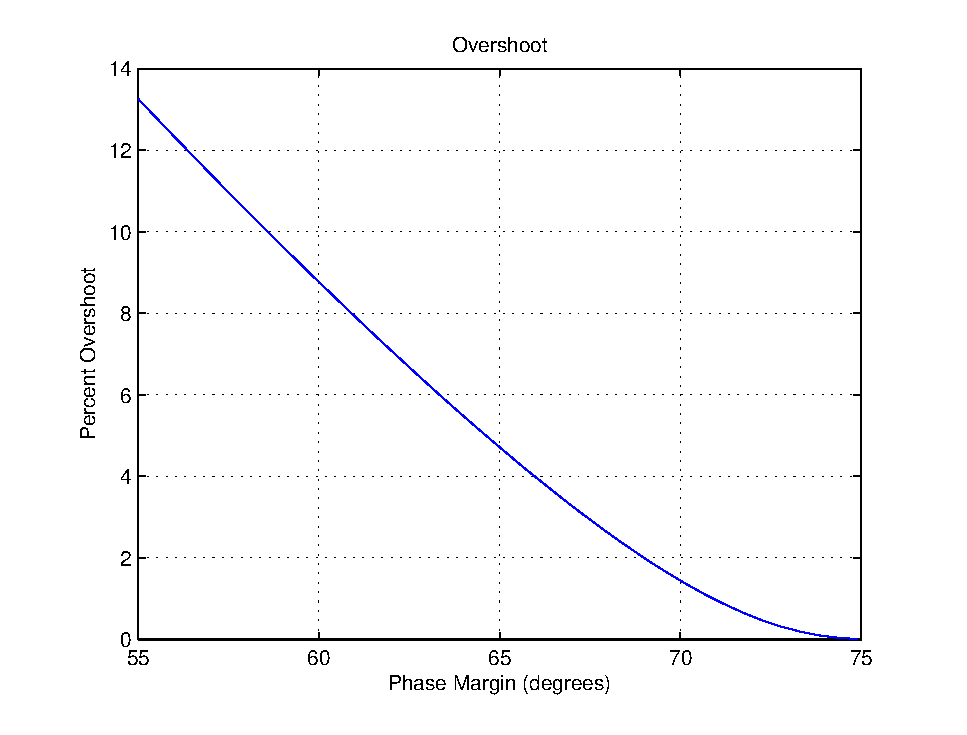
\includegraphics[width=\linewidth]{fig/overshootMargin.eps}
 \caption{Overshoot as a function of the phase margin}
 \label{overshootMargin}
\end{figure}
\end{center}

%------------------------------
% Proportional controller
%------------------------------

\subsubsection*{Proportional controller}

With the PI-controller from the previous section, the ``continuous'' close loop transfer function of the system is:

\begin{equation}
 H_{cl,vel}(p) = \frac{1}{1 + \frac{\tau_m}{K K_m}p}
\end{equation}

Therefore, outputting the position leads to the addition of an integrator block (integration of the velocity). The new transfer function is:

\begin{equation}
 H_{cl,pos}(p) = \frac{1}{p}\frac{1}{1 + \frac{\tau_m}{K K_m}p}
\end{equation}

The maximum rise time for the velocity controller verify $t_{r,vel} \leq 5O \text{ ms} \Leftrightarrow w_c = 125.6 \text{ rad/s}$. Therefore, in the worst case scenario, the transfer function for the position is:

\begin{equation}
 H_{cl,pos}(p) = \frac{1}{p} \frac{1}{1 + \frac{p}{125.6}}
\end{equation}

Figure \ref{bodePos} shows the bode diagram of this function.

\begin{center}
\begin{figure}[ht]
 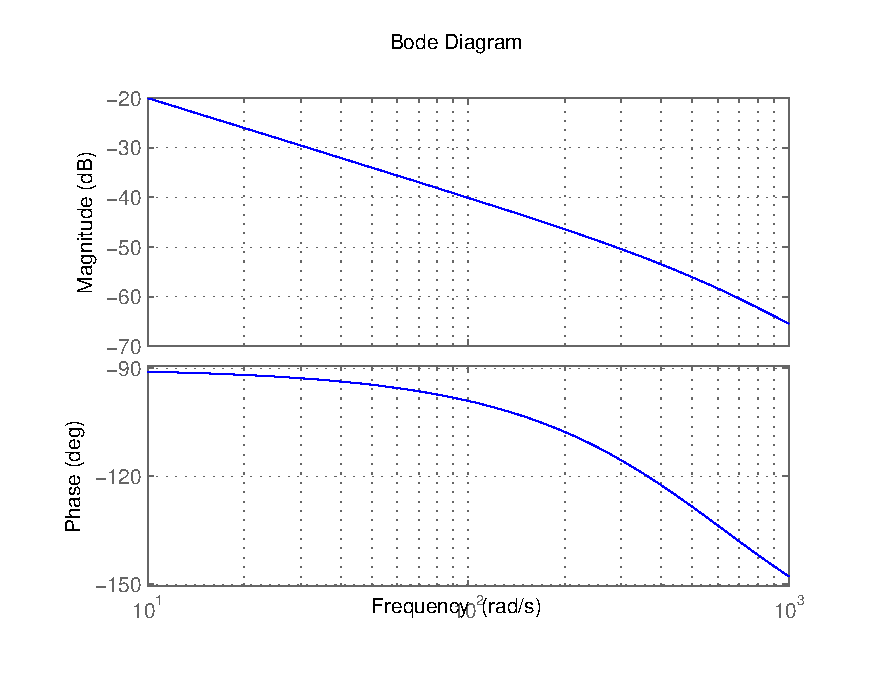
\includegraphics[width=\linewidth]{fig/bodePos.eps}
 \caption{Bode diagram of $H_{cl,pos}$}
 \label{bodePos}
\end{figure}
\end{center}

According to the bode diagram on Figure \ref{bodePos}, we have:

\begin{itemize}
 \item $G_{dB,pos}(\omega = 42.8 \text{ rad/s}) = -32 \text{ dB}$
 \item $\Delta \Phi = 86.3^{\circ}$
\end{itemize}

Therefore, we only need to translate vertically the gain curves in order to fulfill the criteria.

Using a proportional controller $H_{P}(p) = K_P$ leads to:

$$ G_{dB,cont}(\omega = 42.8 \text{ rad/s}) = 32 \text{ dB} \Leftrightarrow K_P = 10^{\frac{32}{20}} = 40$$

Our theoretical proportional controller is:

$$C_{P}(s) = 40$$

Figure \ref{StepPPos} shows the step response of the system. \emph{All of the criteria are met.}

\begin{center}
\begin{figure}[ht]
 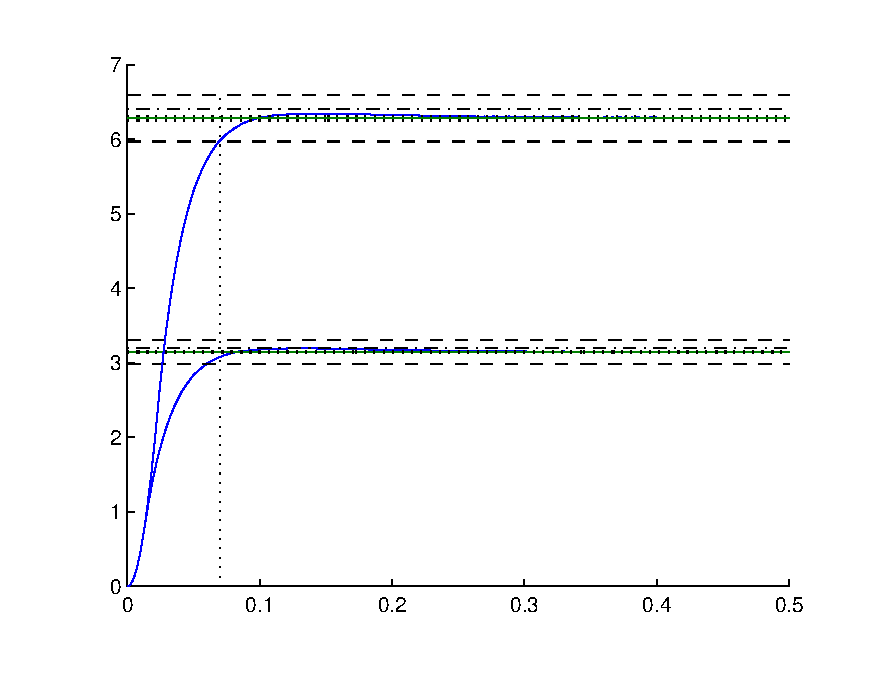
\includegraphics[width=\linewidth]{fig/StepPPos.eps}
 \caption{Steps responses of the system controled in position for two differents amplitudes}
 \label{StepPPos}
\end{figure}
\end{center}



%------------------------------
% Phase advance controller
%------------------------------

\subsubsection*{Phase advance controller}

Whithout any controller, the continuous close loop function of the motor is:

$$ H_{m,pos}(s) = \frac{\frac{K_m}{Rd+K_m}}{1+\frac{RJ}{Rd+K_M K_E}s} \frac{1}{s}$$

Figure \ref{bodePos2} shows the bode diagram of this transfer function.

We want to design a phase advance controller:

$$C_{\Phi}(s) = K_{\Phi} \frac{1 + T_{\Phi}s}{1 + a T_{\Phi} s}, 0 < a < 1$$ 

We want a phase margin equal to $70^{\circ}$ at $\omega_c = 42.8 \text{ rad/s}$. Therefore, since $\Phi_{H_{m,pos}} = 15^{\circ}$, we need $\varphi_m = 45^{\circ}$.

With this kind of controller, $a$ fulfill the following equation:

$$\sin\varphi_m = \frac{1-a}{1+a} \Leftrightarrow a = \frac{1 - \sin\varphi_m}{1 + \sin\varphi_m} = 0.17$$

$T_{\Phi}$ fulfill the following equation:

$$\frac{1}{T_{\Phi}\sqrt{a}} = \omega_c \Leftrightarrow T_{\Phi} = \frac{1}{\omega_c \sqrt{a}} \approx 56 \text{ ms}$$

And $K_{\Phi}$ fulfill the following equation ($\tau_m = \frac{RJ}{Rd+K_M K_E}$): 

\begin{multline*} 20 \log\left(\frac{K}{\sqrt{a}}\right) + |H_{m,pos}(s)|_{\omega = \omega_c} = 0 \\ \Leftrightarrow K_{\Phi} = \frac{\sqrt{a}}{\sqrt{1 + \tau_m \omega_c}} \approx 0.99 \end{multline*}


Our theoretical phase controller is:

$$C_{\Phi}(s) = 0.99 \frac{1 + 0.056s}{1 + 0.0097s} $$



